\documentclass[10pt,a4paper]{amsart}
\usepackage[margin=19mm]{geometry}
\usepackage{amsmath,amssymb,mathtools}
\usepackage[scr=rsfs,cal=euler]{mathalfa}
\usepackage{xfrac}
\usepackage[unicode,hidelinks,bookmarks=false]{hyperref}
\newcommand{\ie}{i.e.\ }
\newcommand{\cf}{cf.\ }
\newcommand{\resp}{respectively\ }
\newcommand{\Subsection}{\subsection}
\providecommand{\nobreakdash}{\nobreak\hbox{-}}
\setlength{\emergencystretch}{2em}
\multlinegap0pt
\usepackage{tikz}
\usepackage{braket}
\usepackage{amssymb}
\newtheorem{theorem}{Theorem}
\newtheorem{scope}{Scope}
\title{Categorical Tensor-Graph Semantics for Quantum Algorithms}
\author{Naihong Hu, Ruining Li, Futao Wang}
\date{Source: arXiv:2607.12128v3 (CC BY 4.0)}
\begin{document}
\maketitle

\noindent\emph{Source and licence.} Categorical Tensor-Graph Semantics for Quantum Algorithms. Version arXiv:2607.12128v3 (CC BY 4.0), distributed by arXiv under the Creative Commons Attribution 4.0 International licence, http://creativecommons.org/licenses/by/4.0/, as recorded in the arXiv licence metadata for this exact version and shown on the abstract page https://arxiv.org/abs/2607.12128v3. Full licence notice: \texttt{licenses/arxiv-2607.12128-CC-BY-4.0.txt}.\par\smallskip

\noindent\textit{Editorial scope.} Counted unit: the article's theorem 5.1 (source0.tex lines 2088--2126). The article's complete original proof of it is delivered with it (source0.tex lines 2323--2389, one \texttt{proof} environment of 67 lines, which the article places away from the statement). No mathematics is written, repaired or re-derived: the statement and the proof are the article's own lines, in the article's own notation, and no retained line is substituted or re-flowed.  Retained uncounted as the source-local context the proof needs: lines 2300--2320; lines 3585--3590.  One declared adaptation: exactly 3 ancillary strings inside the retained spans are omitted (image-inclusion commands and, where the source repeats a label, the repeated label definitions) and no other line differs from the source; the figure environments, with their placement, captions and labels, are kept, and the package records the omitted strings in fidelity receipts bound to the affected bodies.  No retained line contains a citation, so the wrapper carries no bibliography and no bibliography entry.  The retained lines contain the article's own diagram code, which the wrapper typesets with the standard tikz packages; no image file is delivered and the package declares no asset dependency.  Editorial formatting only, in addition: an AMS \texttt{amsart} preamble that restates the article's own declarations and macros used by the retained lines, namely the environments \texttt{theorem}, \texttt{scope} on separate counters, together with the standard packages those lines need.  The retained environments print in this document as Theorem 1, Scope 1 in order of appearance, whereas the article prints the same items with the numbering of its own full document.  The complete native source of the article as distributed in the arXiv e-print for this exact version is bundled unchanged as \texttt{sources/205088/source0.tex}.
\begin{equation}\label{qubit}
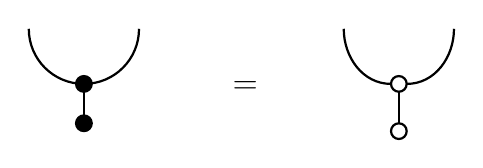
\begin{tikzpicture}[thick]
    \begin{scope}[shift={(0,0)}]
        \draw (0,1.5) to [out=-90,in=180] (0.7,0.8);
        \draw (1.4,1.5) to [out=-90,in=0] (0.7,0.8);
        \node[draw, circle, fill=black, inner sep=2pt] at (0.7,0.8) {};
        \draw (0.7,0.8) -- (0.7,0.3);
        \node[draw, circle, fill=black, inner sep=2pt] at (0.7,0.3) {};
    \end{scope}

    \node at (2.75,0.75) {\large $=$};

    \begin{scope}[shift={(4,0)}]
        \draw (0,1.5) to [out=-90,in=180] (0.6,0.8);
        \draw (1.4,1.5) to [out=-90,in=0] (0.8,0.8);
        \node[draw, circle, fill=white, inner sep=2pt] at (0.7,0.8) {};
        \draw (0.7,0.7) -- (0.7,0.3);
        \node[draw, circle, fill=white, inner sep=2pt] at (0.7,0.2) {};
    \end{scope}
\end{tikzpicture}
\end{equation}

\begin{theorem}[Non-commutative spider theorem]\label{thm2.2}
In a monoidal category, let $(A,  \mu_{B},  \eta_{B},$ $\Delta_{W},  \varepsilon_{W})$ be a Frobenius structure. For any connected morphism $A^{\otimes m} \rightarrow A^{\otimes n}$ built from finitely many $\mu_{B},  \eta_{B},  \Delta_{W},  \varepsilon_{W}$ and $\mathrm{id}$, connected by $\mu_{B},  \eta_{B},  \Delta_{W},  \varepsilon_{W}$, $\mathrm{id}$, $\circ$ and $\otimes$, it is equal to the following normal form:
\begin{center}

\end{center}
\end{theorem}

\begin{theorem}\label{5.1}
In $\mathbf{FHilb}$ and $A=(\mathbb{C}^2)^{\otimes n}$, a pair of complementary symmetric dagger Frobenius structures satisfies:
\begin{center}
%
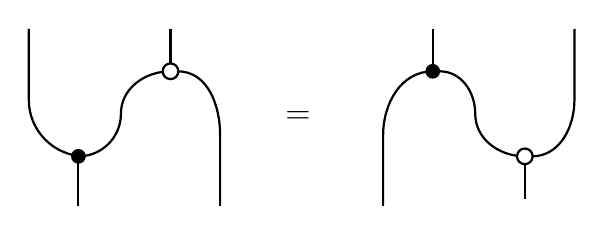
\begin{tikzpicture}[thick, scale=0.9]

    % --- 图 1 (左一) ---
    \begin{scope}[shift={(0,0)}]
        % 左侧输入线下部（修正补全）
        % 这里我根据 basic8 第一张图手绘细节:黑点位于左侧波谷处
        \draw (0,3) -- (0,2) to [out=-90,in=180] (0.8,1.2);
        \draw (0.7,1.2) -- (0.7,0.5); % 黑点下方的线
        \filldraw[black] (0.7,1.2) circle (2.5pt);

        \draw (0.7,1.2) to [out=0,in=-90] (1.3,1.8) to [out=90,in=180] (2,2.4);
        \draw (2,2.4) -- (2,3);
        % 白点:使用 node 遮盖交叉线
        \node[draw, circle, fill=white, inner sep=2pt] at (2,2.4) {};
        \draw (2.1,2.4) to [out=0,in=90] (2.7,1.5) -- (2.7,0.5);
    \end{scope}


    \node at (3.8, 1.75) {\large $=$};

    % --- 图 2 (左二) ---
    \begin{scope}[shift={(5,0)}]
        \draw (0,0.5) -- (0,1.5) to [out=90,in=180] (0.7,2.4);
        \draw (0.7,2.4) -- (0.7,3); % *** Z点上方引线 ***
        \filldraw[black] (0.7,2.4) circle (2.5pt); % 实心黑点
        \draw (0.8,2.4) to [out=0,in=90] (1.3,1.8) to [out=-90,in=180] (2,1.2);
        \draw (2,1.2) -- (2,0.6);
        % 空心白点
        \node[draw, circle, fill=white, inner sep=2pt] at (2,1.2) {};
        \draw (2.1,1.2) to [out=0,in=-90] (2.7,2)-- (2.7,3);
    \end{scope}

\end{tikzpicture}
\end{center}
\end{theorem}

\begin{proof}[Proof of Theorem \ref{5.1}]
\[
%
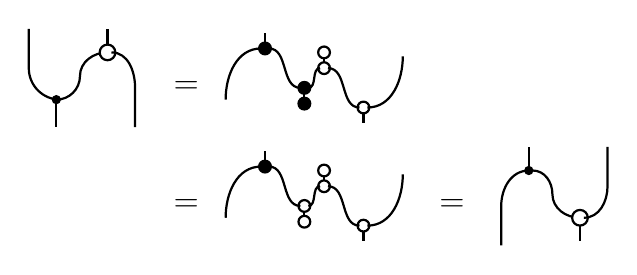
\begin{tikzpicture}[thick, scale=0.5]
    \begin{scope}[shift={(0,0)}]
        % 左侧输入线下部（修正补全）
        % 这里我根据 basic8 第一张图手绘细节:黑点位于左侧波谷处
        \draw (0,3) -- (0,2) to [out=-90,in=180] (0.8,1.2);
        \draw (0.7,1.2) -- (0.7,0.5); % 黑点下方的线
        \filldraw[black] (0.7,1.2) circle (2.5pt);
        \draw (0.7,1.2) to [out=0,in=-90] (1.3,1.8) to [out=90,in=180] (2,2.4);
        \draw (2,2.4) -- (2,3);
        % 白点:使用 node 遮盖交叉线
        \node[draw, circle, fill=white, inner sep=2pt] at (2,2.4) {};
        \draw (2.1,2.4) to [out=0,in=90] (2.7,1.5) -- (2.7,0.5);
    \end{scope}
    \node at (4, 1.5) {\large $=$};
    \begin{scope}[shift={(7,1.5)}]
        \draw (-1,1.1) -- (-1,1.4);
        \draw (0,-0.1) -- (0,-0.3);
        \draw (0.5,0.6) -- (0.5,0.8);
        \draw (1.5,-0.6) -- (1.5,-0.9);
        \node[draw, circle, fill=black, inner sep=1.5pt] at (0,0) {};
        \node[draw, circle, fill=black, inner sep=1.5pt] at (0,-0.4) {};
        \node[draw, circle, fill=black, inner sep=1.5pt] at (-1,1) {};
        \node[draw, circle, fill=white, inner sep=1.5pt] at (0.5,0.5) {};
        \node[draw, circle, fill=white, inner sep=1.5pt] at (0.5,0.9) {};
        \node[draw, circle, fill=white, inner sep=1.5pt] at (1.5,-0.5) {};
        \draw (-2,-0.3) to [out=90,in=180] (-1.1,1);
        \draw (-0.9,1) to [out=0,in=180] (-0.1,0);
        \draw (0.1,0) to [out=0,in=180] (0.4,0.5);
        \draw (0.6,0.5) to [out=0,in=180] (1.4,-0.5);
        \draw (1.6,-0.5) to [out=0,in=-90] (2.5,0.8);
    \end{scope}
    \node at (4, -1.5) {\large $=$};
    \begin{scope}[shift={(7,-1.5)}]
        \draw (-1,1.1) -- (-1,1.4);
        \draw (0,-0.1) -- (0,-0.3);
        \draw (0.5,0.6) -- (0.5,0.8);
        \draw (1.5,-0.6) -- (1.5,-0.9);
        \node[draw, circle, fill=white, inner sep=1.5pt] at (0,0) {};
        \node[draw, circle, fill=white, inner sep=1.5pt] at (0,-0.4) {};
        \node[draw, circle, fill=black, inner sep=1.5pt] at (-1,1) {};
        \node[draw, circle, fill=white, inner sep=1.5pt] at (0.5,0.5) {};
        \node[draw, circle, fill=white, inner sep=1.5pt] at (0.5,0.9) {};
        \node[draw, circle, fill=white, inner sep=1.5pt] at (1.5,-0.5) {};
        \draw (-2,-0.3) to [out=90,in=180] (-1.1,1);
        \draw (-0.9,1) to [out=0,in=180] (-0.1,0);
        \draw (0.1,0) to [out=0,in=180] (0.4,0.5);
        \draw (0.6,0.5) to [out=0,in=180] (1.4,-0.5);
        \draw (1.6,-0.5) to [out=0,in=-90] (2.5,0.8);
    \end{scope}
    \node at (10.75, -1.5) {\large $=$};
    \begin{scope}[shift={(12,-3)}]
        \draw (0,0.5) -- (0,1.5) to [out=90,in=180] (0.7,2.4);
        \draw (0.7,2.4) -- (0.7,3); % *** Z点上方引线 ***
        \filldraw[black] (0.7,2.4) circle (2.5pt); % 实心黑点
        \draw (0.8,2.4) to [out=0,in=90] (1.3,1.8) to [out=-90,in=180] (2,1.2);
        \draw (2,1.2) -- (2,0.6);
        % 空心白点
        \node[draw, circle, fill=white, inner sep=2pt] at (2,1.2) {};
        \draw (2.1,1.2) to [out=0,in=-90] (2.7,2)-- (2.7,3);
    \end{scope}
\end{tikzpicture}
\]
\noindent where the first and third equalities both use the non-commutative spider theorem \ref{thm2.2}, and the second equality uses \ref{qubit} .
\end{proof}

\end{document}
